% =============================================================================
% Working extract -- Results, Q3 section, redraft 2026-08-23 (fourth pass).
% NOT full prose yet -- phrase-level building blocks per the agreed workflow:
% claim -> numbers (source) -> how tested -> ruled out -> caveat -> figure/table -> so-what.
% Do not write full sentences from this until each block is signed off.
% Source of truth for every number: temp_results_pinn/RESULTS_TABLE.md (live-verified,
% not the brain dump prose, which may lag). Cross-reference before promoting any number here.
%
% FOURTH-PASS CHANGE: 2c substantially rewritten. Was "PINN's biggest flaw traces to one
% place." Now leads with a real, convergent, cross-model finding -- the personalisation
% captures a genuine two-sided productivity signal (over- AND under-productive sites),
% verified against independent yield-class records (checked: yldc is NOT a model input,
% and is independently recorded, not derived from this project's own height measurements --
% see chat, 2026-08-23). The plain-PINN-vs-PINN-k plausibility difference is now framed as
% "how each variant expresses the same real signal," not a standalone flaw. Section 3 gains
% a new point: PINN-k is measurably safer/more realistic, not just more complete. Figures:
% two are still being finalised (the compartment map and hotspot-summary map may be merged
% or replaced; the "same plot, two models" curve figure is proposed but not yet built) --
% flagged clearly below, do not treat as final.
% =============================================================================

\section{Q3: Prediction and physics guidance}
\label{sec:results-q3}

\subsection{Results}

% --- Table 1: six-model comparison (unchanged, existing) ---
% [Existing Table~\ref{tab:results-q3} -- see current main draft, not reproduced here.]

% --- Table 2: PINN/PINN-k across feature sets and hyperparameter checks (unchanged) ---
\begin{table}[!htbp]
\centering
\small
\begin{tabular}{lrr}
\toprule
Condition & PINN $R^2$ & PINN-$k$ $R^2$ \\
\midrule
\multicolumn{3}{l}{\textit{Feature set}} \\
No environment & 0.573 & 0.573 \\
Set2 (small list) & $0.627\pm0.023$ & $0.622\pm0.017$ \\
Set3 (medium list, headline) & $0.631\pm0.027$ & $0.618\pm0.023$ \\
Set4 (large list) & $0.618\pm0.029$ & $0.620\pm0.020$ \\
\midrule
\multicolumn{3}{l}{\textit{Hyperparameters}} \\
Main result (Set3, reported settings) & 0.631 & 0.618 \\
Learning-rate check & 0.630 & 0.614 \\
Batch-size check & 0.641 & 0.619 \\
Lambda check (8 settings, range) & 0.623--0.632 & 0.612--0.620 \\
\bottomrule
\end{tabular}
\caption{\small{...}} % caption TBD; source: RESULTS_TABLE.md #5, #3, #3b, #4
\label{tab:pinn-conditions}
\end{table}

% --- Table 3: compartment 1129 cross-fold check (unchanged) ---
\begin{table}[!htbp]
\centering
\small
\begin{tabular}{lrrr}
\toprule
Fold & Split membership & Mean $y_{max}$ deviation & Rows $>$70\,m (of 1484) \\
\midrule
0 & 100\% test & $+12.1$\,m & 72 \\
1 & 95\% train & $+11.5$\,m & 44 \\
2 & 98\% train & $+10.7$\,m & 0 \\
3 & 100\% train & $+15.6$\,m & 0 \\
4 & 100\% validation & $+12.4$\,m & 0 \\
\bottomrule
\end{tabular}
\caption{\small{...}} % caption TBD; source: RESULTS_TABLE.md #10
\label{tab:compartment1129-crossfold}
\end{table}

% --- Table 4: trunk-residual comparison, plain PINN vs. PINN-k (unchanged) ---
\begin{table}[!htbp]
\centering
\small
\begin{tabular}{lrrr}
\toprule
Fold & Plain PINN trunk mean$|\cdot|$ & PINN-$k$ trunk mean$|\cdot|$ & Ratio \\
\midrule
0 & 0.207 & 0.410 & 1.98$\times$ \\
1 & 0.238 & 0.553 & 2.33$\times$ \\
2 & 0.255 & 0.844 & 3.31$\times$ \\
\bottomrule
\end{tabular}
\caption{\small{...}} % caption TBD; source: RESULTS_TABLE.md #7
\label{tab:trunk-residual}
\end{table}

% --- Table 5: error by age band and height band (unchanged) ---
\begin{table}[!htbp]
\centering
\small
\begin{tabular}{lrrrr}
\toprule
Age band (years) & $n$ & DNN MAE & PINN MAE & PINN-$k$ MAE \\
\midrule
15--30 & 13,338 & 2.50 & 2.53 & 2.51 \\
30--45 & 21,879 & 3.12 & 3.13 & 3.22 \\
45--60 & 7,919 & 4.13 & 3.84 & 4.16 \\
60--75 & 1,973 & 5.06 & 5.28 & 5.48 \\
75--93 & 923 & 6.16 & 6.59 & 7.01 \\
\midrule
Height band & $n$ & DNN MAE & PINN MAE & PINN-$k$ MAE \\
\midrule
0--10\,m & 4,874 & 3.43 & 4.28 & 4.05 \\
10--20\,m & 18,796 & 2.94 & 2.83 & 2.82 \\
20--30\,m & 17,949 & 3.11 & 3.02 & 3.28 \\
30--47\,m & 4,413 & 5.01 & 4.74 & 5.09 \\
\bottomrule
\end{tabular}
\caption{\small{...}} % caption TBD; source: RESULTS_TABLE.md #12
\label{tab:age-height-error}
\end{table}

% --- Table 6 (NEW): over- and under-productive compartments, both models ---
\begin{table}[!htbp]
\centering
\small
\begin{tabular}{llrrl}
\toprule
Compartment & Direction & Yield class & $n$ plots & Flagged by \\
\midrule
1129 & Over-productive & 22--24 & 371 & Plain PINN ($y_{max}$) + PINN-$k$ ($k$) \\
2229 & Over-productive & 24 & 6 & Plain PINN + PINN-$k$ \\
2219 & Over-productive & -- & -- & PINN-$k$ ($k$) only, not yet checked in plain PINN \\
\midrule
2031 & Under-productive & 12 & 406 & Plain PINN ($y_{max}$) + PINN-$k$ ($k$) \\
2142 & Under-productive & 8 (mostly), 16 & 394 & Plain PINN + PINN-$k$ \\
\bottomrule
\end{tabular}
\caption{\small{...}} % caption TBD; source: chat 2026-08-23 (compartment hotspot check + master data join)
\label{tab:productivity-compartments}
\end{table}

% --- Table 7 (NEW): correlation with independent yield-class records ---
\begin{table}[!htbp]
\centering
\small
\begin{tabular}{lrr}
\toprule
Comparison & Pearson $r$ & $n$ \\
\midrule
Plain PINN $y_{max}$ deviation vs.\ yield class & 0.249 & 11,508 \\
PINN-$k$'s $k$ vs.\ yield class & 0.234 & 11,508 \\
PINN-$k$'s $y_{max}$ vs.\ yield class & 0.334 & 11,508 \\
\bottomrule
\end{tabular}
\caption{\small{...}} % caption TBD -- note: yldc confirmed NOT a model input (checked against
% both the terrain feature list and the no-env feature list) and independently recorded
% (Forest Research inventory, not derived from this project's own height measurements).
% Source: chat 2026-08-23.
\label{tab:yieldclass-correlation}
\end{table}

% --- Table 8 (NEW): plausibility comparison, plain PINN vs. PINN-k ---
\begin{table}[!htbp]
\centering
\small
\begin{tabular}{lrr}
\toprule
& Plain PINN $y_{max}$ deviation & PINN-$k$ $y_{max}$ deviation \\
\midrule
Mean & $+2.93$\,m & $-0.23$\,m \\
SD & 5.32\,m & 0.72\,m \\
Max & $+25.79$\,m & $+1.05$\,m \\
Implausible ($<$5\,m or $>$70\,m) & 18 / 11,508 (0.16\%) & 0 / 11,508 (0\%) \\
\bottomrule
\end{tabular}
\caption{\small{...}} % caption TBD; source: RESULTS_TABLE.md #2, chat 2026-08-23
\label{tab:plausibility-comparison}
\end{table}

% --- Figures ---
% STATUS NOTE: figures below are mixed built/pending -- two are still being finalised and
% may be replaced or merged before this goes further. Flagged individually.

\begin{figure}[!htbp]
\centering
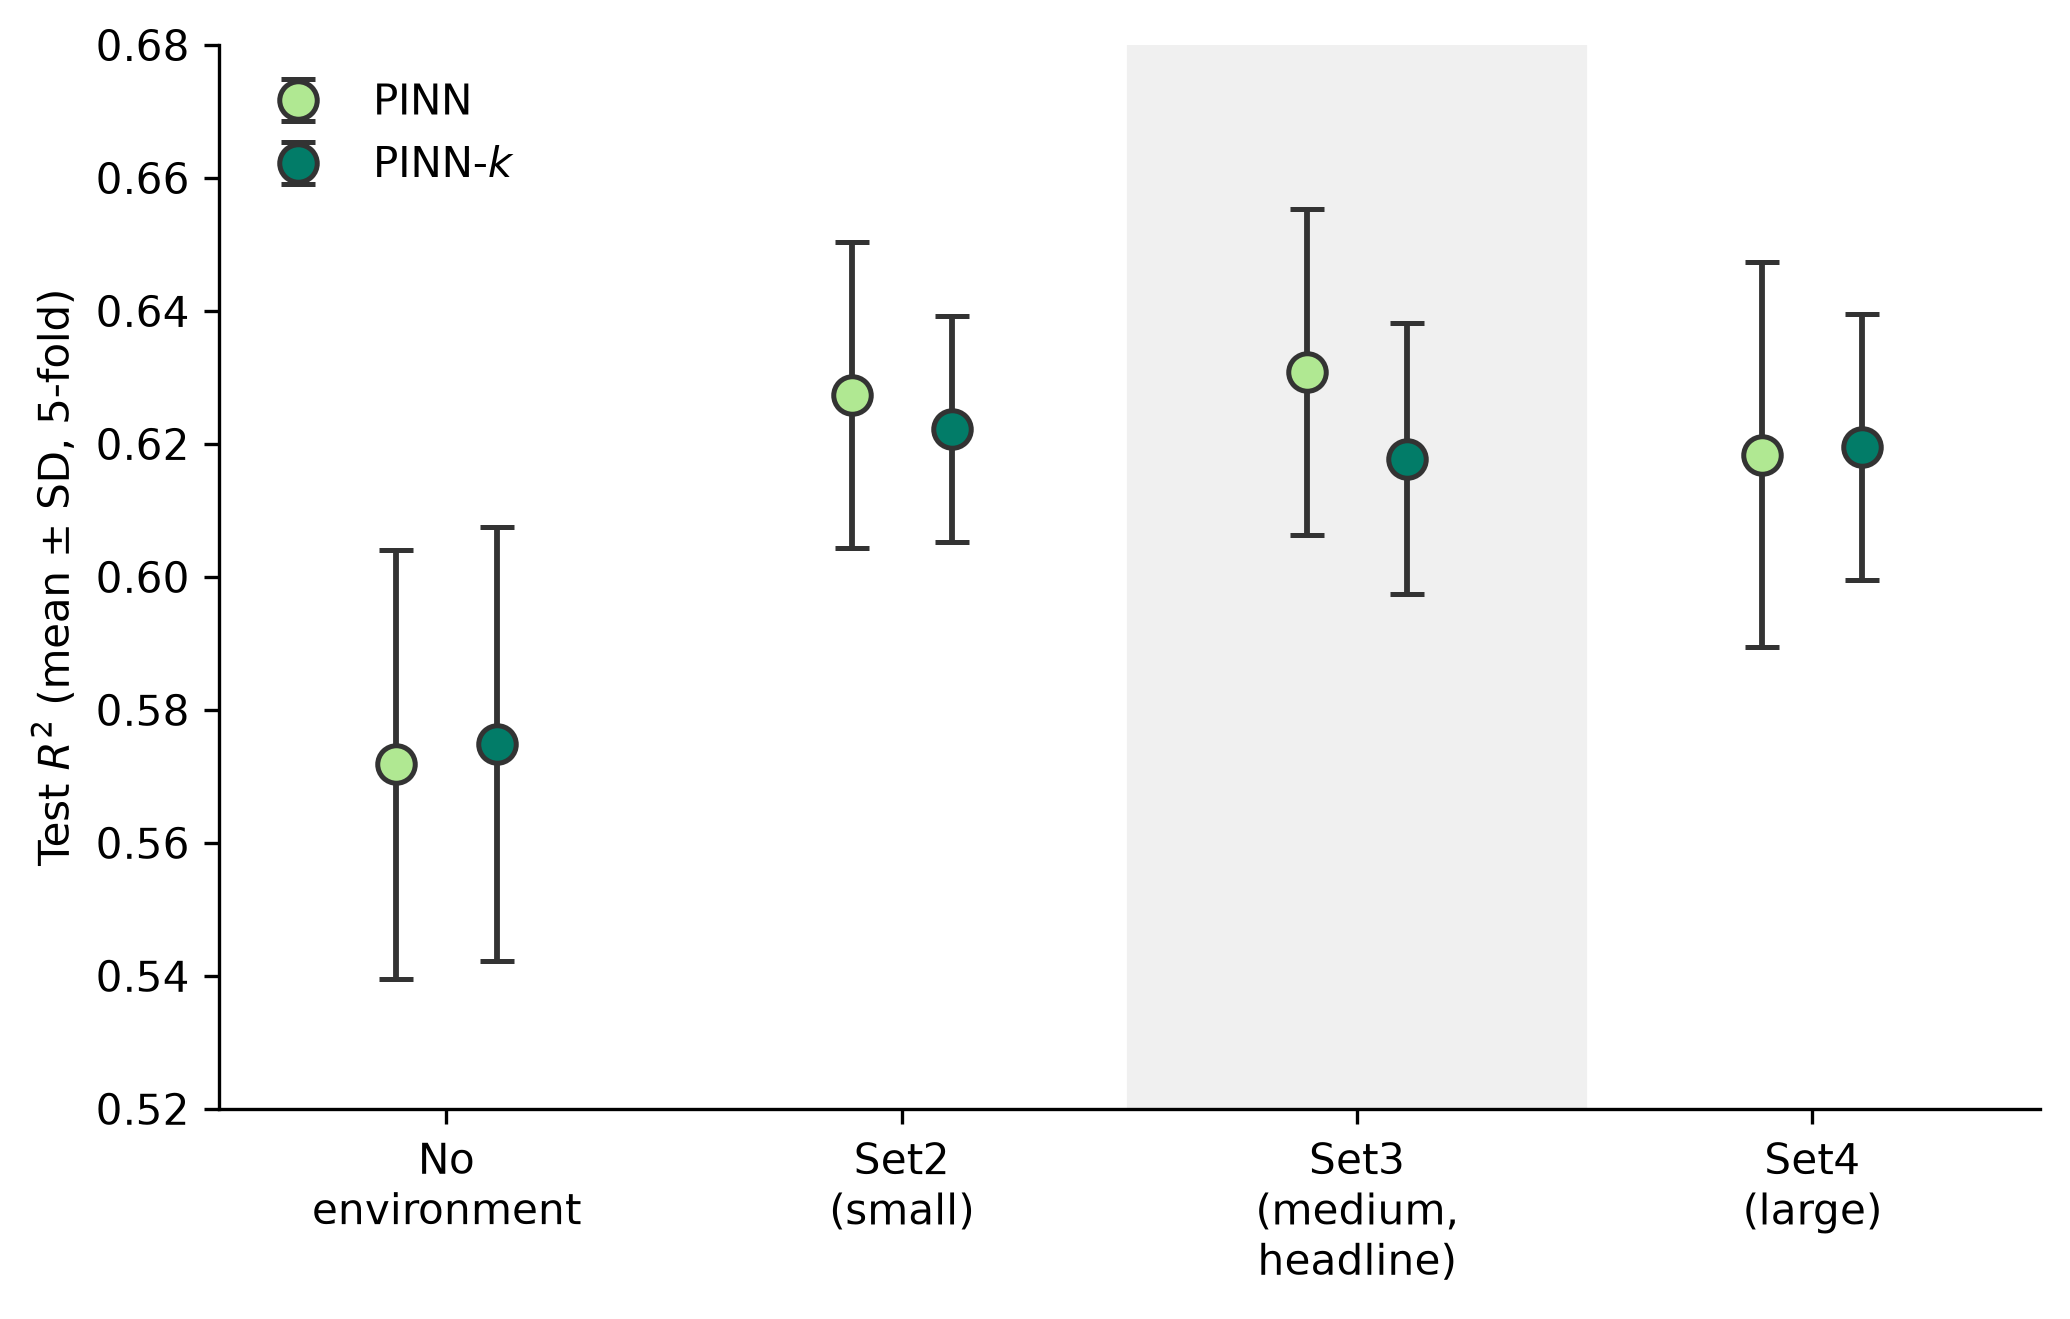
\includegraphics[width=0.75\textwidth]{figures/fig_results/q3_env_sweep_r2.png}
\caption{\small{PINN and PINN-$k$ accuracy against environmental feature-list size.}}
% BUILT, stable. Source: RESULTS_TABLE.md #5. MAIN TEXT.
\label{fig:env-sweep}
\end{figure}

\begin{figure}[!htbp]
\centering
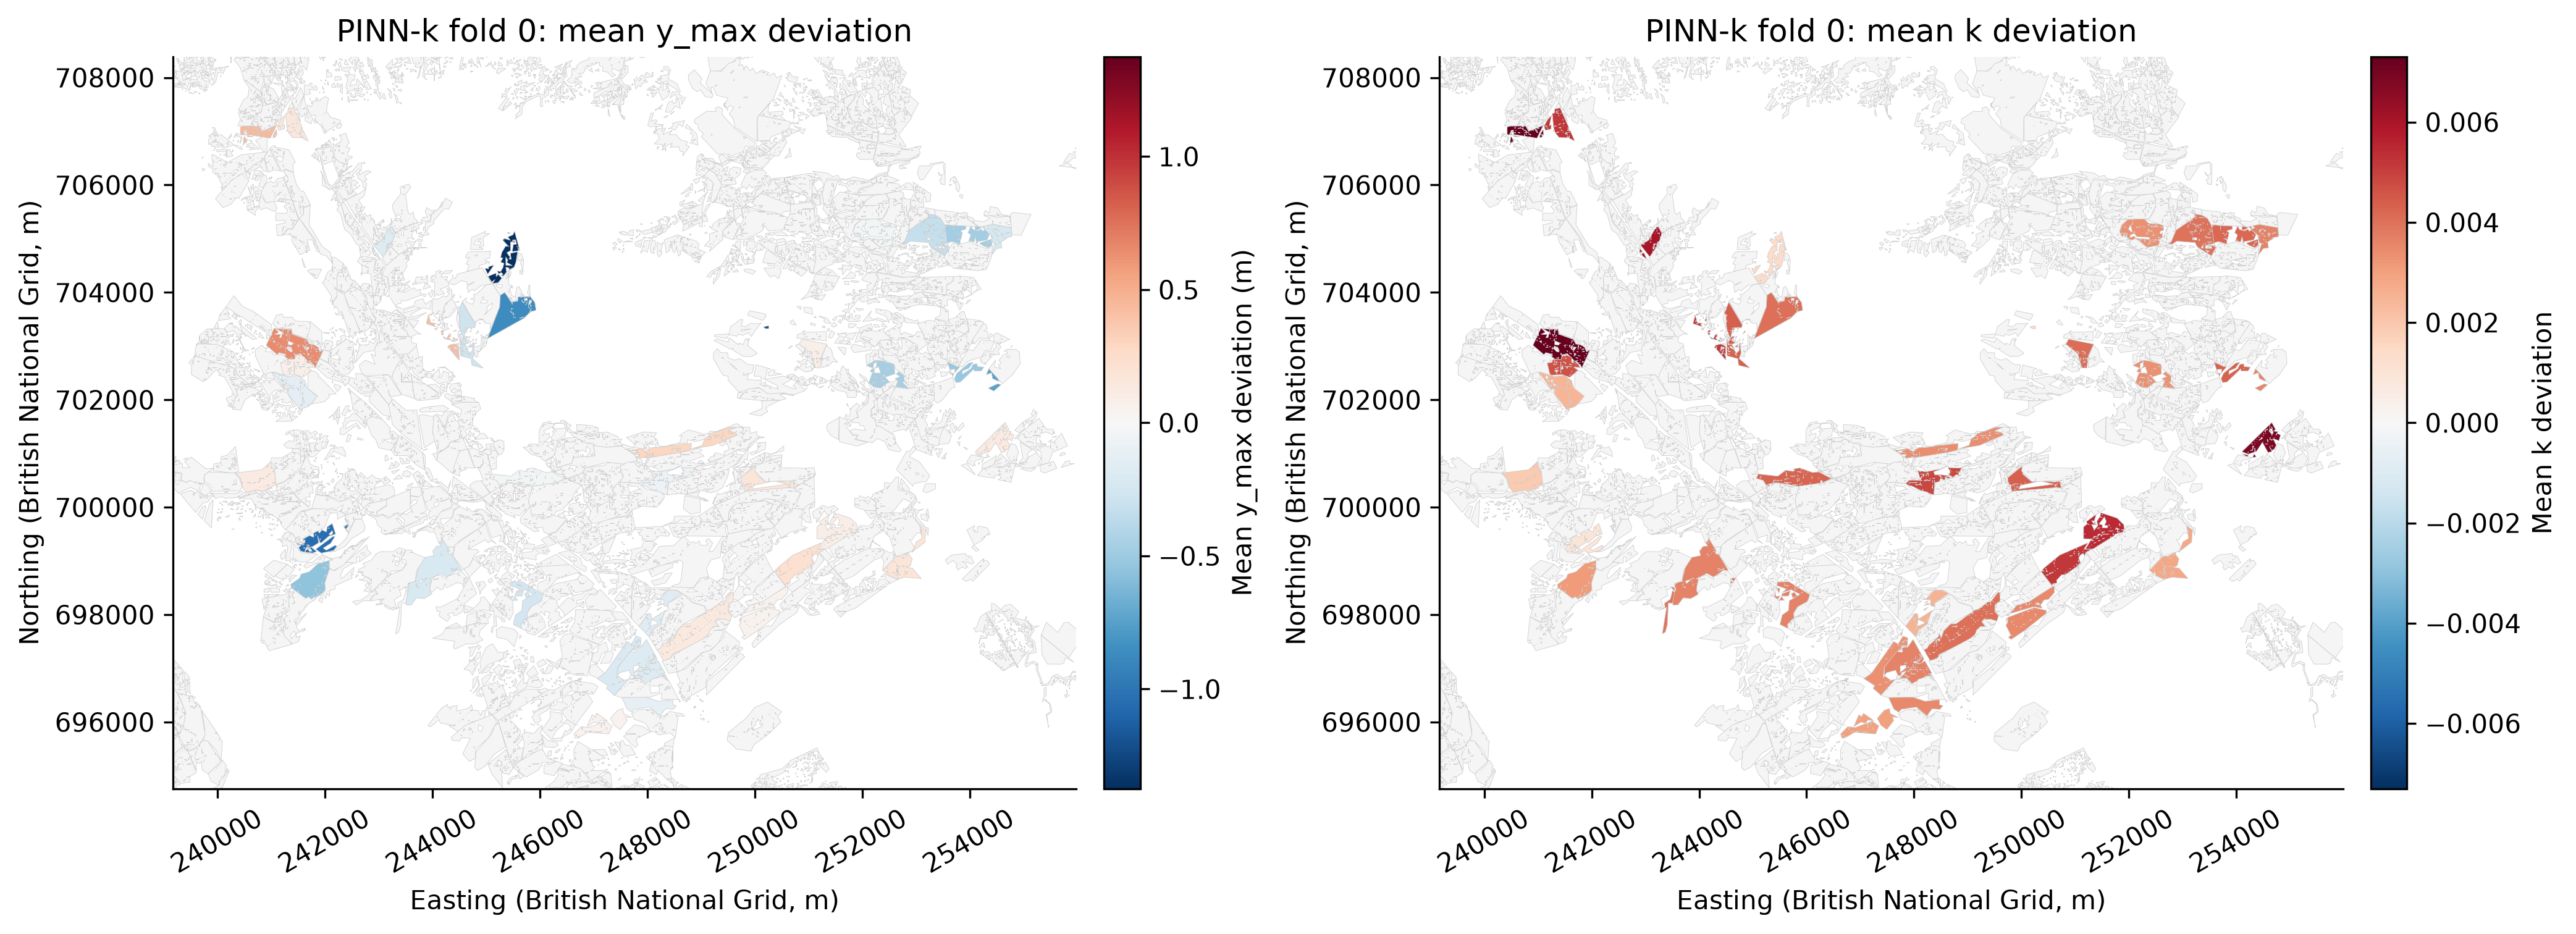
\includegraphics[width=0.9\textwidth]{figures/fig_results/q3_pinn_k_fold0_ymax_k_deviation_maps.png}
\caption{\small{PINN-$k$, fold 0: mean $y_{max}$ deviation (left) vs.\ mean $k$ deviation
(right), by compartment. $y_{max}$ stays close to flat almost everywhere; $k$ shows the
structured hotspot pattern instead -- the same underlying signal, routed through a
different parameter than plain PINN uses.}}
% BUILT. Directly shows the parameter-routing finding. MAIN TEXT -- likely the single most
% important new figure given the 2c rewrite. Source: chat 2026-08-23.
\label{fig:ymax-k-deviation-maps}
\end{figure}

\begin{figure}[!htbp]
\centering
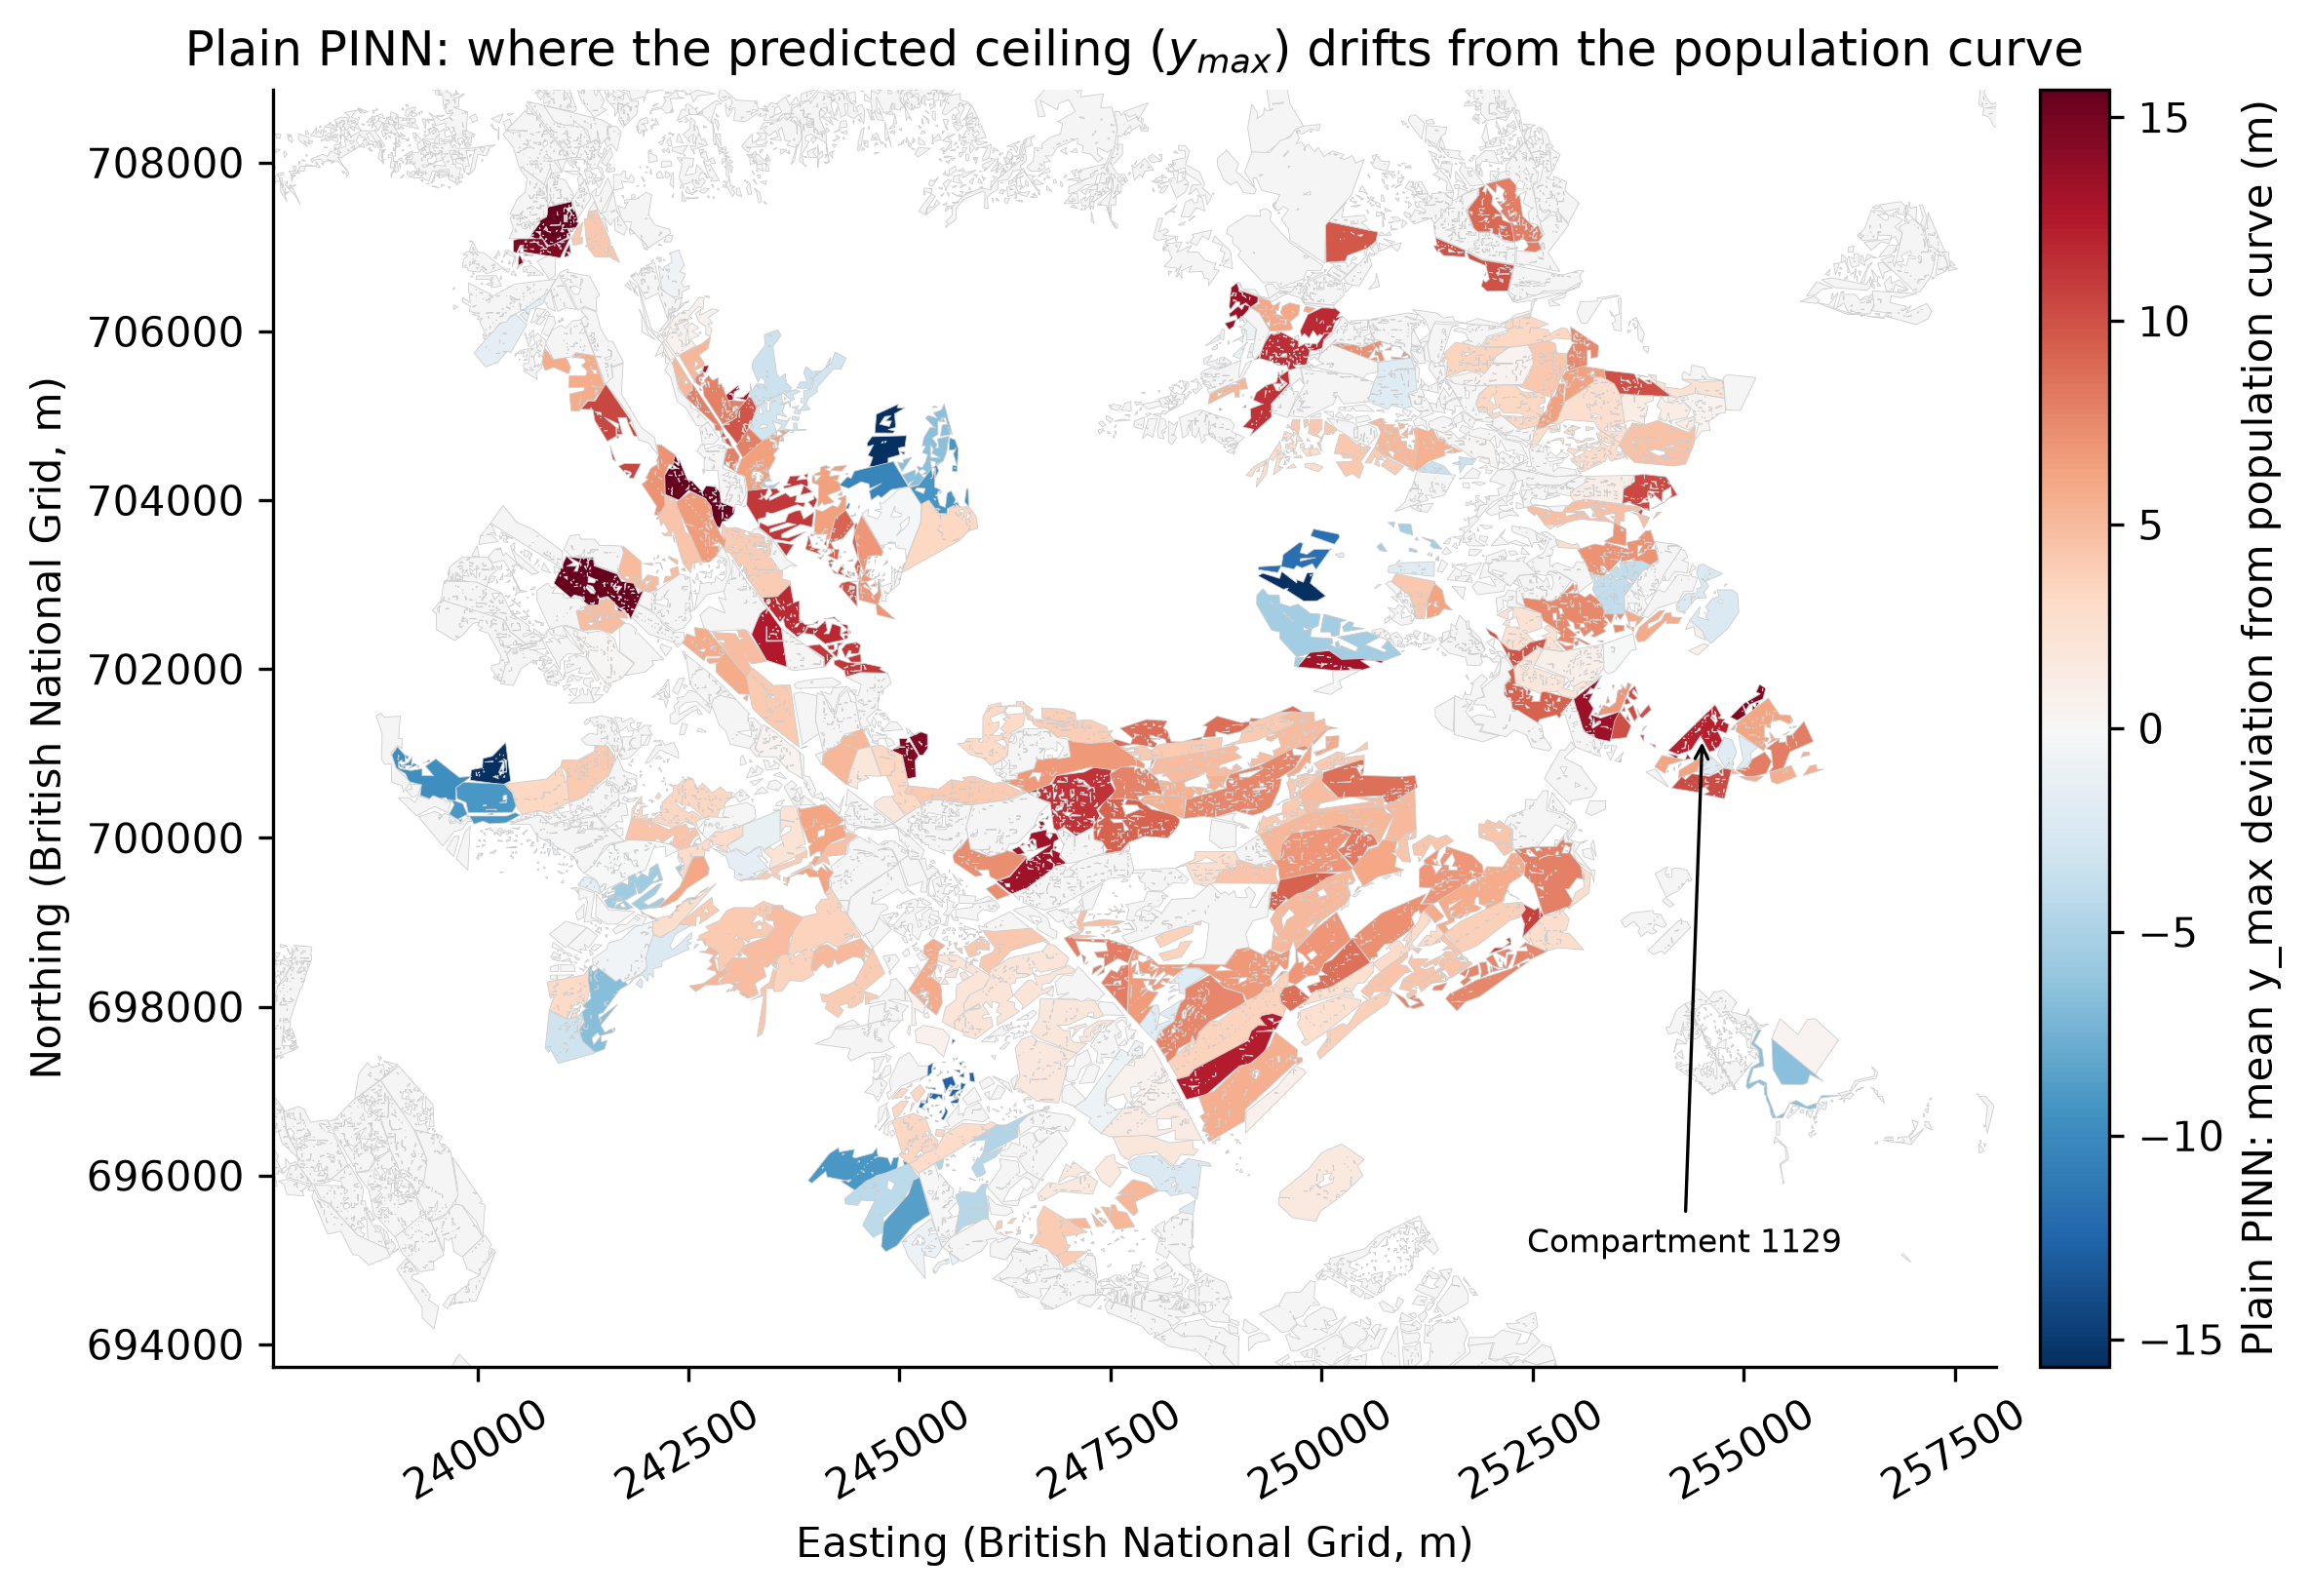
\includegraphics[width=0.8\textwidth]{figures/fig_results/q3_pinn_ymax_deviation_map.png}
\caption{\small{Plain PINN: mean $y_{max}$ deviation from the population curve, by
compartment, pooled across all 5 folds.}}
% BUILT but STATUS UNSETTLED -- may be replaced/paired with q3_pinn_ymax_hotspot_summary.png
% (labels all 5 top hotspots, not just 1129) depending on which reads better once 2c is
% rewritten to cover multiple compartments, not just 1129. MAIN TEXT for now.
\label{fig:ymax-deviation-map}
\end{figure}

\begin{figure}[!htbp]
\centering
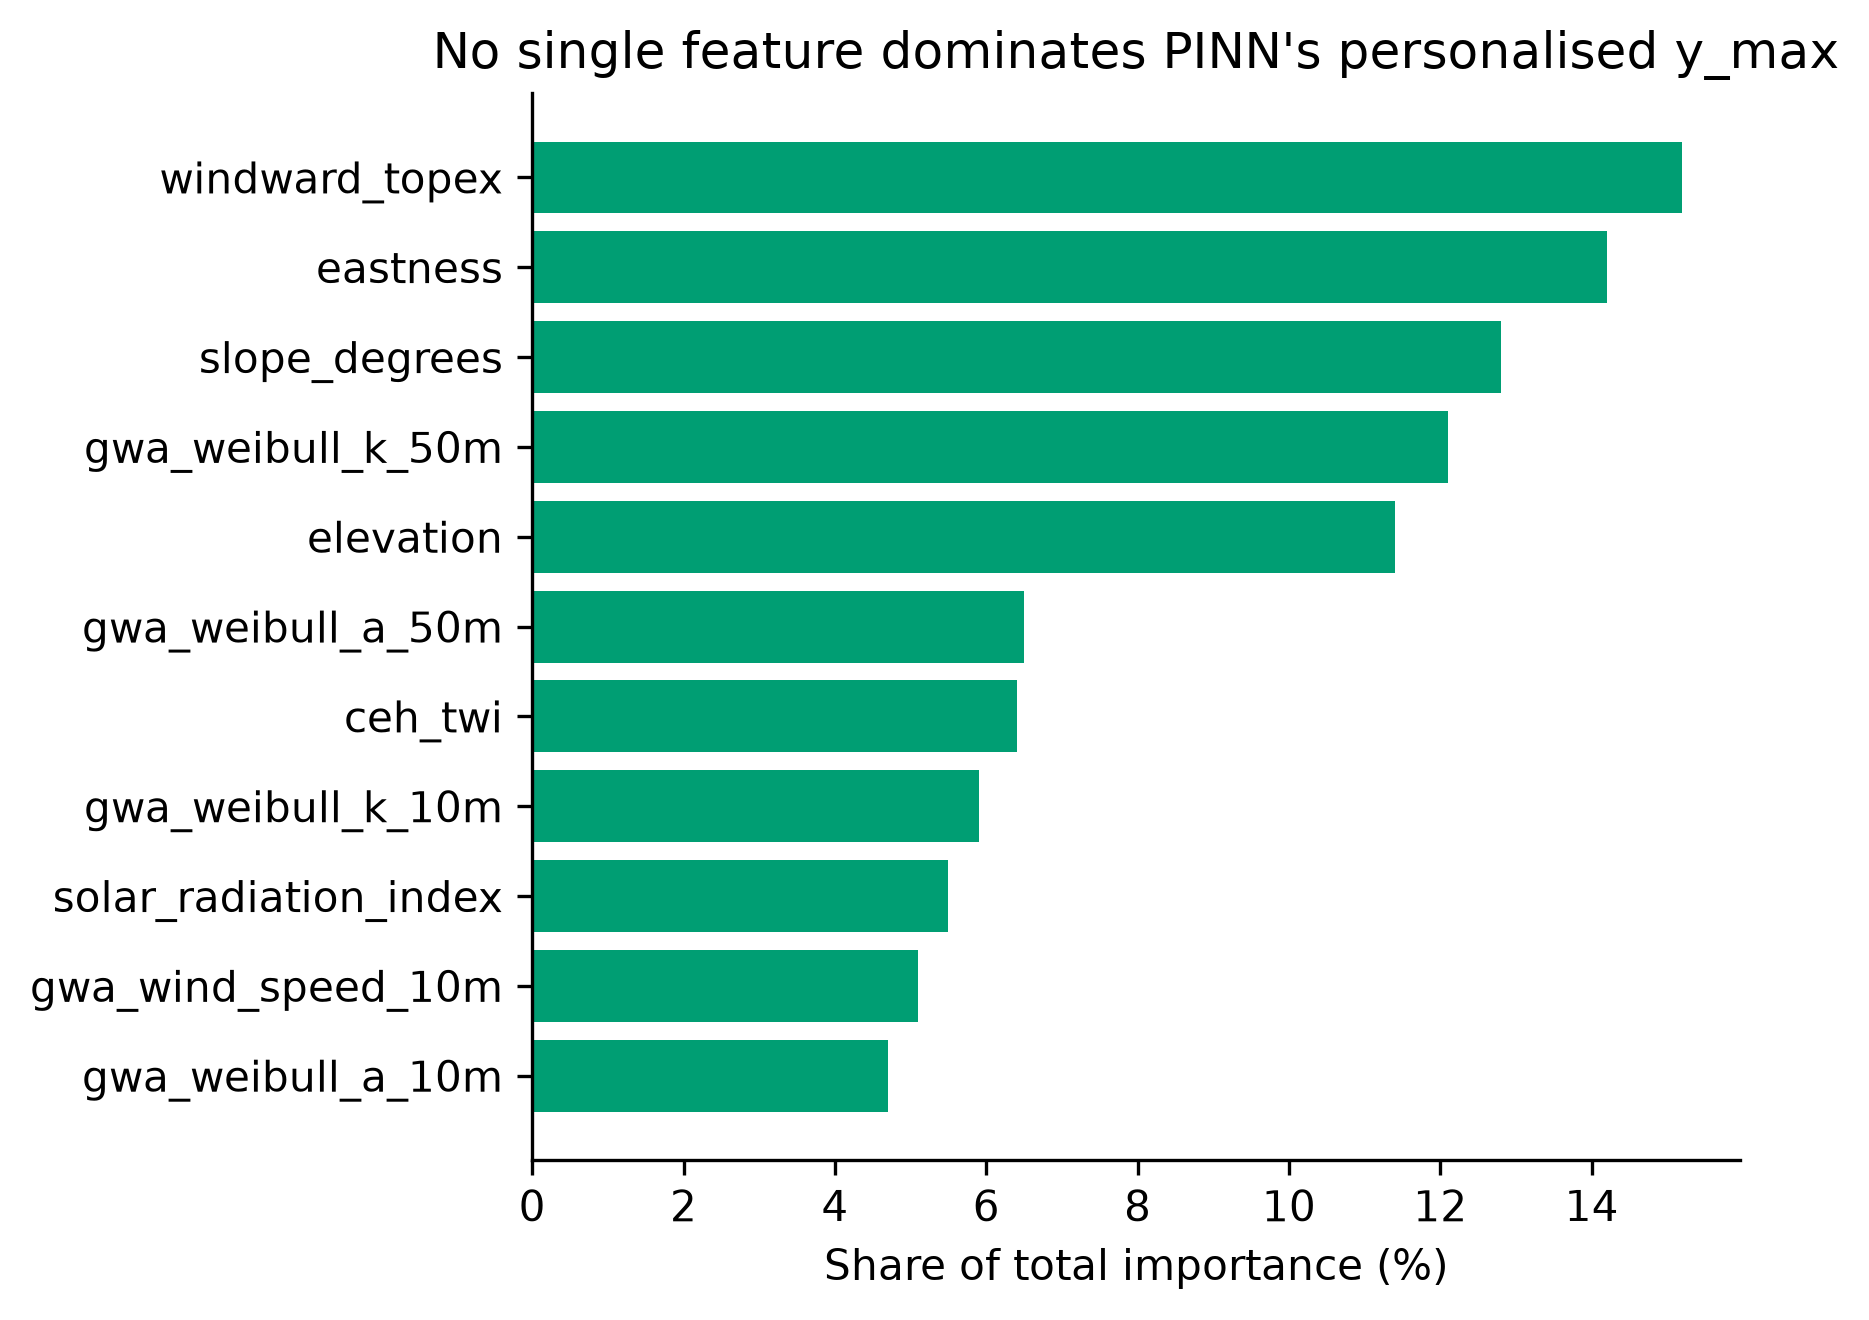
\includegraphics[width=0.7\textwidth]{figures/fig_results/q3_pinn_terrain_importance.png}
\caption{\small{Share of total permutation importance carried by each terrain/wind feature
in PINN-$k$'s personalised $y_{max}$, fold 0.}}
% BUILT, stable. APPENDIX. Source: RESULTS_TABLE.md #6.
\label{fig:terrain-importance}
\end{figure}

\begin{figure}[!htbp]
\centering
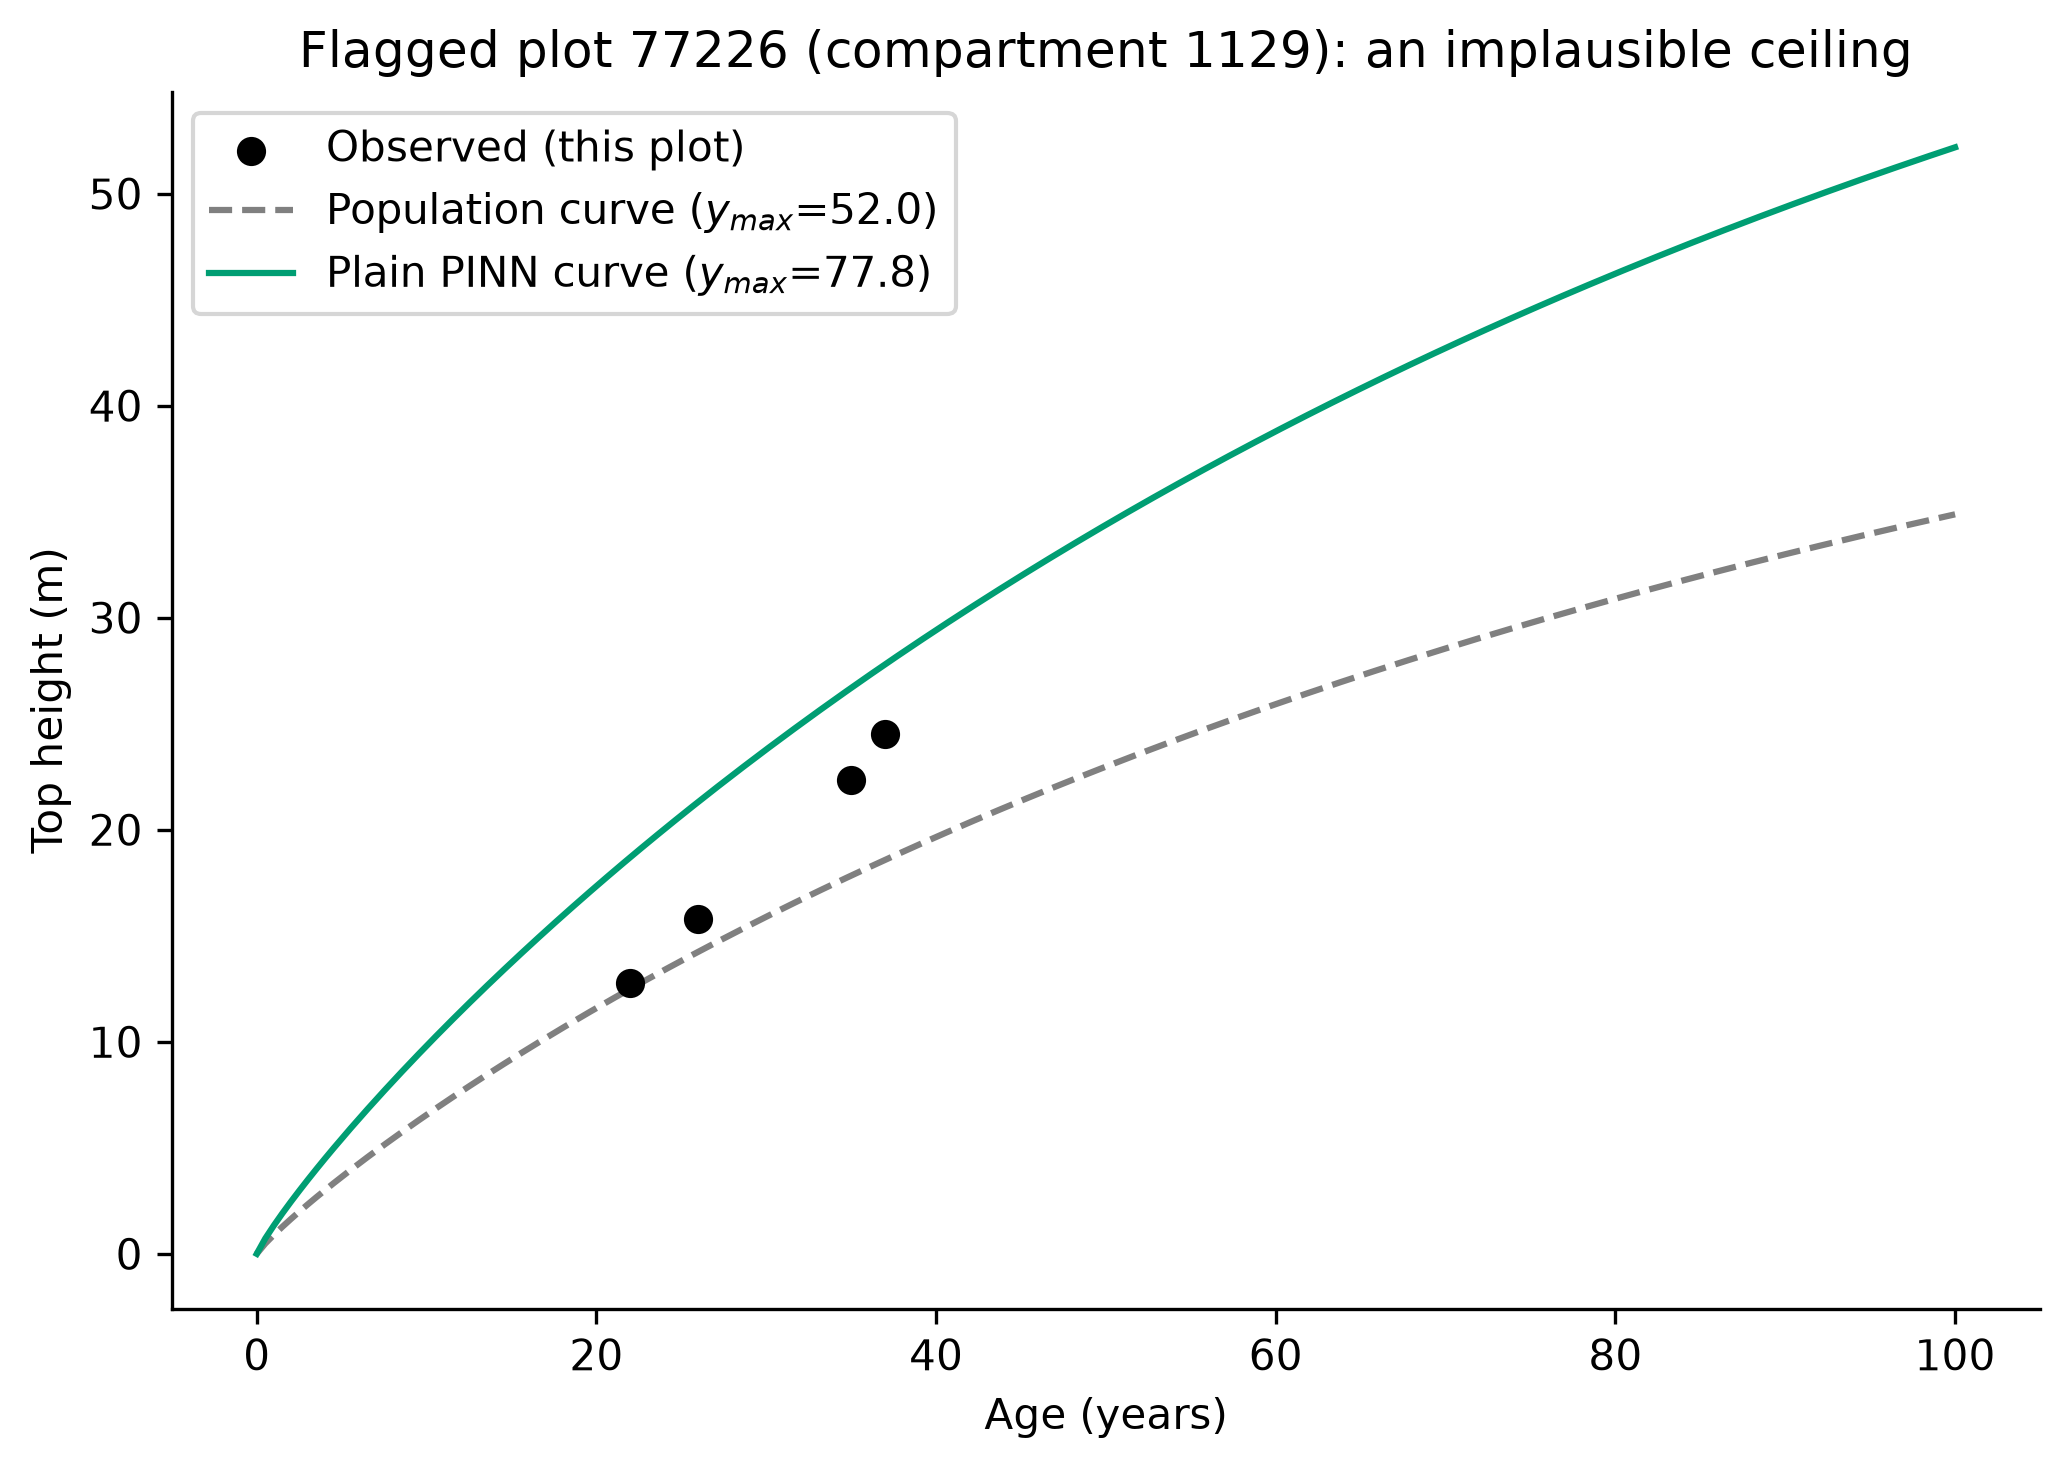
\includegraphics[width=0.7\textwidth]{figures/fig_results/q3_pinn_implausible_example_plot.png}
\caption{\small{Plot 77226 (compartment 1129): observed heights, the population curve, and
plain PINN's personalised curve.}}
% BUILT but a candidate for replacement -- proposed alternative shows the SAME plot with
% BOTH plain PINN's curve (wild) and PINN-k's curve (modest, plausible) against the same
% population baseline, directly visualising the parameter-routing finding at the single-plot
% level. Not yet built. Decide before finalising: keep this version, or replace with the
% two-model version. APPENDIX either way.
\label{fig:implausible-example}
\end{figure}

\begin{figure}[!htbp]
\centering
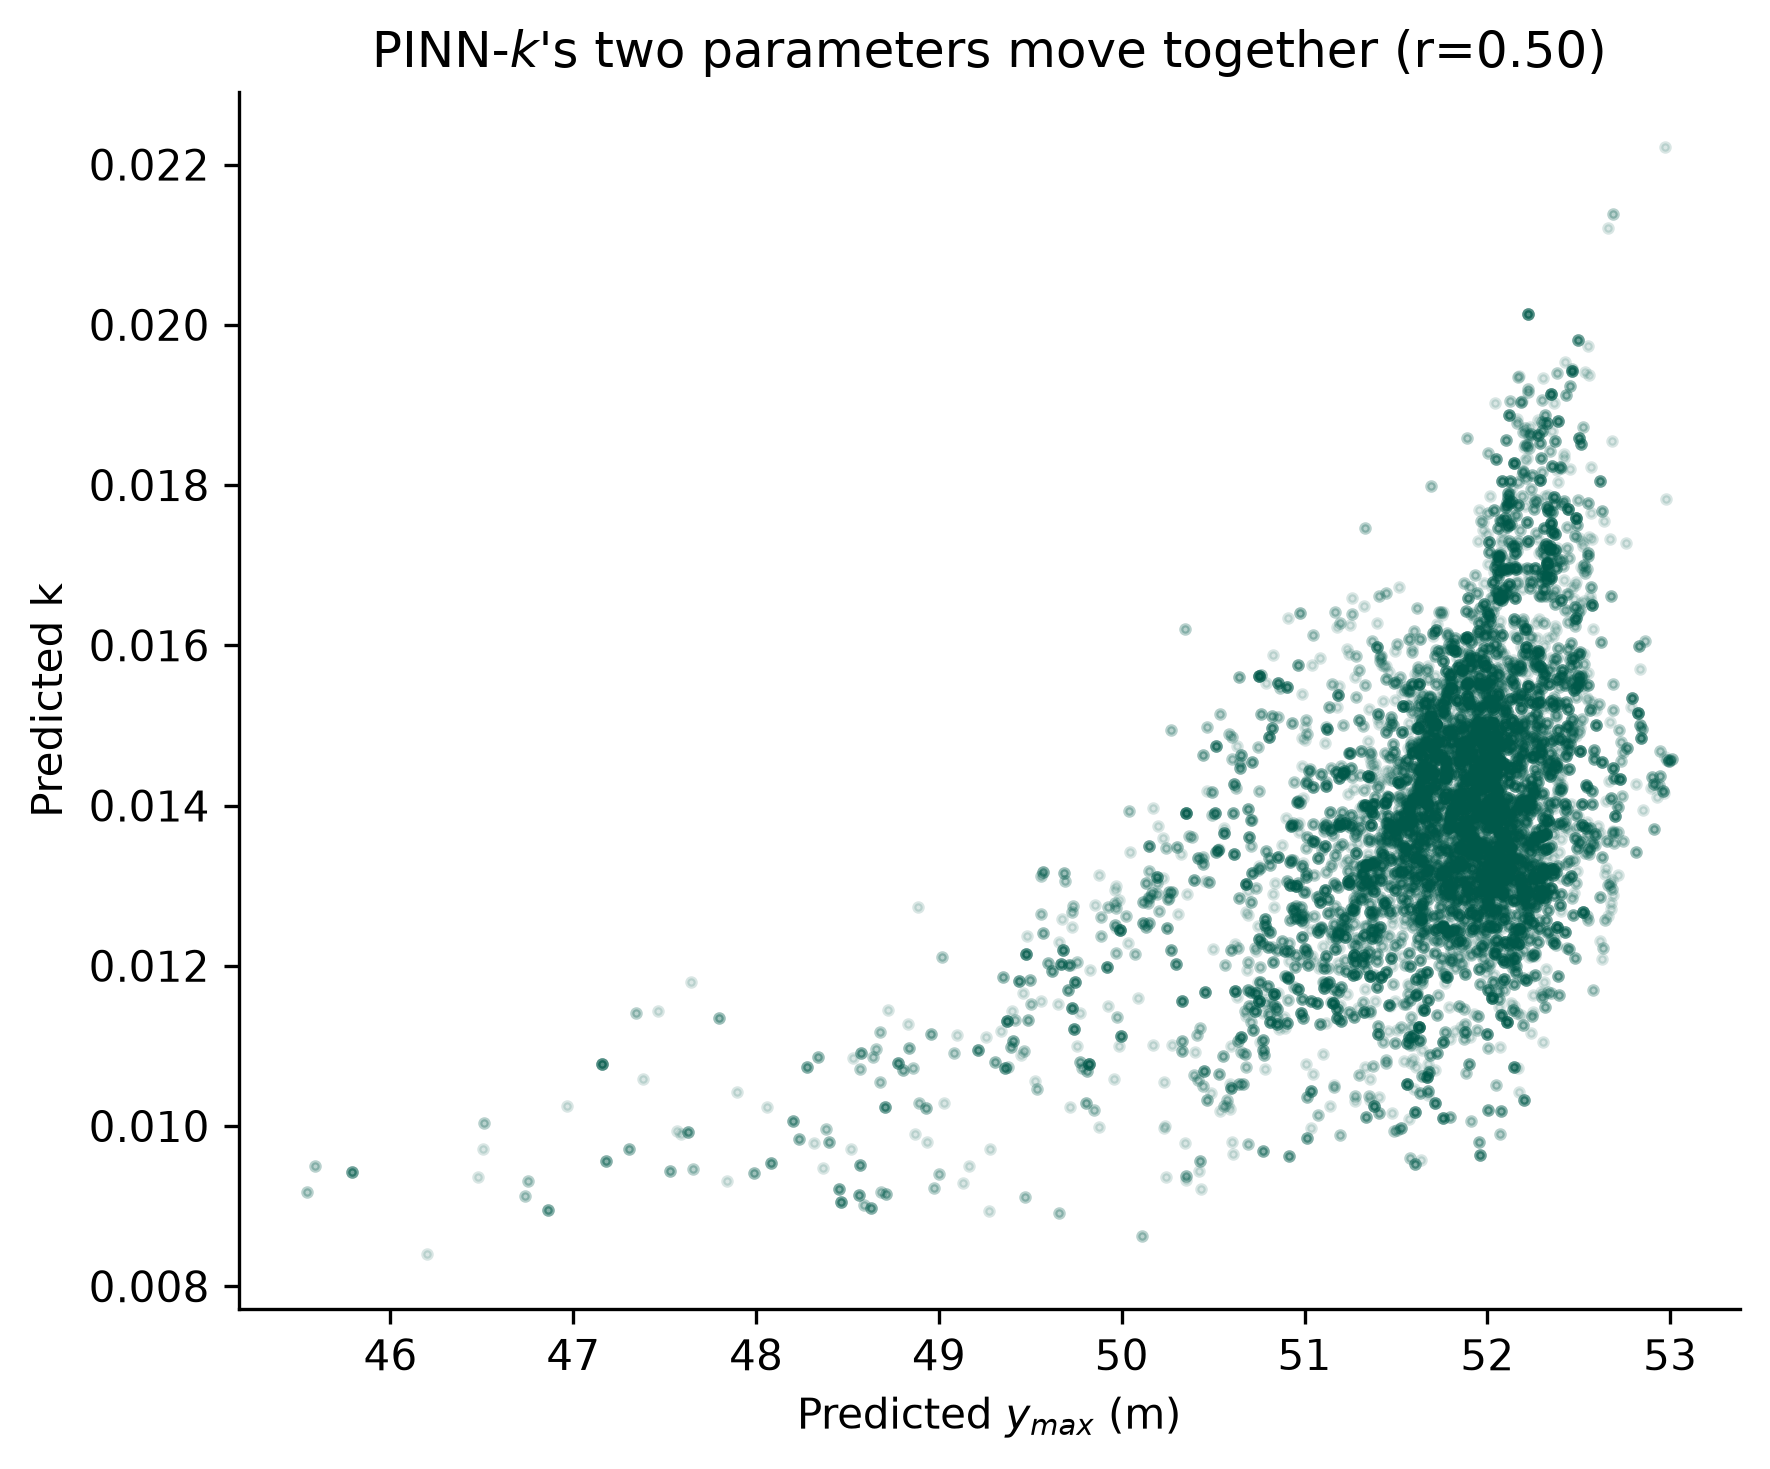
\includegraphics[width=0.65\textwidth]{figures/fig_results/q3_pinn_ymax_k_scatter.png}
\caption{\small{PINN-$k$'s two personalised parameters, one dot per test-set plot.}}
% BUILT, stable. APPENDIX. Source: chat 2026-08-23 (r=0.50).
\label{fig:ymax-k-scatter}
\end{figure}

\subsection{Discussion}

% -----------------------------------------------------------------------------
% 1. PIVOT (folded-in, NOT its own section/heading) -- unchanged.
% -----------------------------------------------------------------------------

\paragraph*{Trees still win on raw accuracy.}
XGBoost most accurate, DNN close behind, PINN and PINN-$k$ both trail
(Table~\ref{tab:results-q3}).
Four possible reasons checked for DNN's gap to XGBoost. All ruled out: feature interactions,
compartment count, network size, unfamiliar terrain.
Training settings checked again this session, at the correct batch size. Same result. Gap
stands.
Real question: does PINN still earn its place, despite losing here?

% -----------------------------------------------------------------------------
% 2. IS PINN'S INTERPRETABILITY GENUINE? -- unchanged shape (2a real -> 2b driven by real
% signal -> 2c honest about where it breaks), but 2c is substantially rewritten.
% -----------------------------------------------------------------------------

% --- 2a. The personalisation is real, not one variable in disguise -- unchanged ---

\paragraph*{The personalisation is real, not one hidden variable.}
Checked whether one terrain feature secretly drives the prediction. Same problem Q2 found in
a different model.
Shuffled each feature, one at a time, ten repeats each. Watched how much the prediction moved
(Figure~\ref{fig:terrain-importance}).
No single feature dominates. Top feature, wind exposure, carries 15.2\% of the total. All
eleven span 4.7\%--15.2\%.
Q2's model (GNNWR) leaned on one variable, CanopyCover, for 80--90\% of its signal. This model
does not.
One fold checked so far. Not yet repeated on others -- flagged, not hidden.

% --- 2b. The thing driving it is real (environment sweep) -- unchanged ---

\paragraph*{Environment helps a lot -- once. More does not help further.}
Tested PINN with no environment information, then three feature lists, small to large. Five-
fold CV throughout (Table~\ref{tab:pinn-conditions}, Figure~\ref{fig:env-sweep}).
Zero environment info to a small list: a real, solid jump, several times the fold-to-fold
noise floor.
A bigger list on top of that: no further gain, slightly hurts the simpler version. A
well-chosen list beats a big one.
This fixes a broken earlier test -- the pre-fix code showed no difference between having
environment information or not at all, a bug, not a real result.
One caveat: the headline list is not proven best for the two-parameter version -- the smaller
list scores marginally higher, within normal noise.
Checked why the big list does not help. Its extra features are not ignored -- more than their
fair share of the model's attention -- they just do not carry over to new stands as well.

% --- 2c. REWRITTEN: the personalisation tells a real, two-sided story ---

\paragraph*{The personalisation tells a real story about which sites are more, and less,
productive -- checked against independent records.}
A small number of compartments get pushed well above the population curve. A small number get
pushed well below it. Not random -- the same compartments show up in both PINN and PINN-$k$,
even though the two models express it through different parameters
(Figure~\ref{fig:ymax-k-deviation-maps}).
One compartment (1129, 371 plots) carries most of the extreme high predictions in plain PINN.
The same compartment carries the single highest growth-rate value in PINN-$k$, even though its
personalised height there is unremarkable (Table~\ref{tab:productivity-compartments}).
A mirror pair (2031, 2142, around 400 plots each) shows the same pattern in reverse -- pushed
down in both models.
Checked against the forestry service's own yield-class records -- recorded independently,
never seen by either model. The over-productive compartments carry yield class 22--24, near
the top of the whole range. The under-productive pair carry yield class 8--12, near the
bottom.
Checked this is not just three cherry-picked compartments: a real, significant correlation
holds across the whole test set, not just the extremes (Table~\ref{tab:yieldclass-correlation}).
Modest, not dominant -- yield class explains part of the picture, not most of it. Terrain
(2a) is still doing most of the work.

\paragraph*{The two PINN versions differ in how safely they express the same signal.}
Plain PINN sometimes pushes the signal too far -- a small number of plots reach a height no
real tree does. PINN-$k$ never does this (Table~\ref{tab:plausibility-comparison}).
Plain PINN has only one outlet for this signal, the ceiling itself. PINN-$k$ has two, and
mostly uses growth rate instead, leaving the ceiling close to the shared curve.
Checked this is not a held-out generalisation problem, the same way as before: trained on the
compartment's own real data in four of five folds, the inflated prediction did not shrink --
if anything it grew (Table~\ref{tab:compartment1129-crossfold}).
What is left unresolved: a real, unusually strong or weak site, or a fault in how some of
these places' heights were recorded. Both still open, though the yield-class match makes the
first explanation more likely than it looked before.

\paragraph*{The same weakness still shows up at the extremes of age and height.}
Checked whether mistakes cluster by tree age or height, across all three models, same
held-out rows (Table~\ref{tab:age-height-error}).
Young and mid-range ages: all three models close, sometimes the simpler PINN slightly ahead.
Oldest ages and shortest stands: DNN clearly best, PINN-$k$ the worst of the three.
Not resolved by anything above. A personal curve, fit mostly to well-observed ages, does not
stretch well to the extremes -- the same mechanism as compartment 1129's implausible cases,
now shown as a general pattern, not fixed by having a second parameter available.

% So-what / practical link (still a discussion point, not drafted into prose):
% top height feeds directly into volume (Vol95 = g1 x Top_Height95^g3 x area/10000 x
% CanopyCover, g3~1.48-1.69 for Sitka Spruce) and into General Yield Class via the same
% Chapman-Richards site-index inversion this project's models are built on -- height errors
% are AMPLIFIED downstream into volume, why a disclosed, understood failure mode matters
% practically, not just academically.

% -----------------------------------------------------------------------------
% 3. PLAIN PINN VS. PINN-K: THE RECOMMENDATION -- gains a new safety point.
% -----------------------------------------------------------------------------

\paragraph*{The simpler PINN wins on accuracy. The two-parameter version buys a fuller,
and safer, picture.}
Compared the two versions everywhere -- final height only, vs.\ final height and growth speed.
Simpler version wins every time, a small but consistent gap, across four separate checks
(Table~\ref{tab:pinn-conditions}).
Tried one reason to prefer the two-parameter version anyway: convert its growth-speed number
into a yield class foresters already use. Did not hold up, an old quirk in that formula, not
something this model found. Dropped.
Two real reasons remain. A fuller picture: final height and how fast a stand gets there, not
just one number. And a safer one: the two-parameter version never produces an implausible
height, where the simpler version occasionally does (Table~\ref{tab:plausibility-comparison}).
Checked why the extra parameter costs accuracy. The shared correction network works
increasingly harder in the two-parameter version, across every fold checked
(Table~\ref{tab:trunk-residual}). Growth speed does not fit cleanly by itself; something else
has to compensate. The two parameters do move together sensibly, though
(Figure~\ref{fig:ymax-k-scatter}) -- not fitting independently to noise.

% -----------------------------------------------------------------------------
% 4. WHY TRUST THESE NUMBERS -- closing methods note, not a headline. Unchanged.
% -----------------------------------------------------------------------------

\paragraph*{The settings were checked, not guessed.}
Learning rate, batch size, and physics-weighting strength each tested against other values
(Table~\ref{tab:pinn-conditions}). None beat what was already reported.
Plain PINN still wins under every one. Not a one-setting fluke.
